\documentclass[a4paper, 10pt]{article}
%\usepackage[utf8]{inputenc}			
\usepackage[english]{babel}		% for german	
\usepackage{graphicx}								
\usepackage{parskip}
\usepackage{listings}
\usepackage{xcolor}
\usepackage{amsmath}
\usepackage{mathtools}
\usepackage{amssymb}
\usepackage{mathrsfs}
\usepackage{empheq}
\usepackage{titlesec}	
\usepackage{tikz}
\usetikzlibrary{arrows, snakes,shapes}
%\usepackage{tabularx}
%\usepackage{pdfpages}
%\usepackage{hyperref,breakurl}
%\usepackage{url}
%\usepackage{psfrag}
\usepackage{epstopdf}
\usepackage{dsfont}
\usepackage{sectsty}
\allsectionsfont{\bfseries\sffamily}

\addtolength{\textwidth}{2.1cm}
\addtolength{\topmargin}{-1.4cm}
\addtolength{\oddsidemargin}{-1.1 cm}
\definecolor{leichtgrau}{gray}{0.91}
\setlength{\parindent}{0pt}

% \lstset{language = C,
	% basicstyle=\footnotesize,       
	% numbers=left,                  
	% numberstyle=\footnotesize,      
	% stepnumber=2,
	% numbersep=5pt,
	% backgroundcolor=\color{leichtgrau},
	% frame=single,
% }

% Definition von römischen Zahlen
\makeatletter
\newcommand{\rmnum}[1]{\romannumeral #1}
\newcommand{\Rmnum}[1]{\expandafter\@slowromancap\romannumeral #1@}
\makeatother
%\renewcommand{\familydefault}{\sfdefault}


\begin{document}
\setcounter{section}{2}
\section{Multiuser MIMO}
\begin{itemize}
	\item We distinguish two cases:
	\begin{itemize}
		\item multipoint\,-\,to\,-\,point transmission
		\item point\,-\,to\,-\,multipoint transmission
	\end{itemize}
	\item Multipoint\,-\,to\,-\,point transmission
	\begin{itemize}
		\item typical uplink scenario in cellular systems
		\item information theoretical channel model: Multiple Access Channel (MAC)
		\begin{figure}[h]\centering
			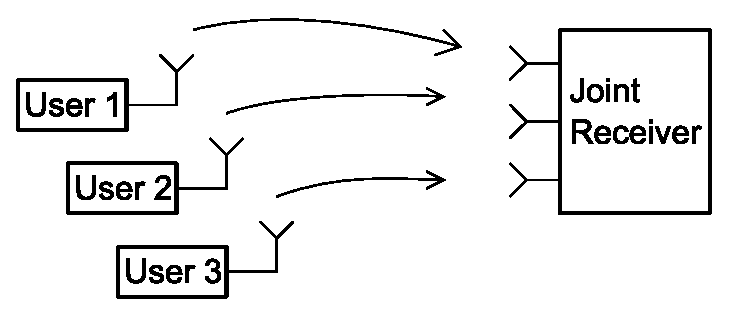
\includegraphics[scale=0.8]{MAC}
		\end{figure}
%		\begin{tikzpicture}
%			\node (user1) at (0,0) [draw] {User 1};
%			\node (user2) at (1,-1)[draw] {User 2};
%			\node (user3) at (2,-2)[draw] {User 3};		
%			\draw[-<] (user1.east) --(1,0) --(1,0.5);        
%			\draw[-<] (user2.east) --(2,-1) --(2,-0.5); 
%			\draw[-<] (user3.east) --(3,-2) --(3,-1.5); 
%			\node[draw, minimum width = 2cm, minimum height = 2.5cm, font = \bfseries\large] (Joint_Receiver) at (10,-1) {Joint Receiver};
%			\path[draw,-<] ([xshift = 0cm, yshift = 0.5cm] Joint_Receiver.west)--([xshift = -1cm, yshift = 0.5cm] Joint_Receiver.west);
%			\path[draw,-<] (Joint_Receiver.west)--([xshift = -1cm, yshift = 0cm] Joint_Receiver.west) ;
%			\path[draw,-<] ([xshift = 0cm, yshift = -0.5cm] Joint_Receiver.west)--([xshift = -1cm, yshift = -0.5cm] Joint_Receiver.west);
%			\path[draw,->,>=stealth'] ([xshift = 0.6cm,yshift = 0.4cm] user1.east)--([xshift = -2.5cm, yshift = 0.5cm] Joint_Receiver.west);
%			\path[draw,->,>=stealth'] ([xshift = 0.6cm,yshift = 0.4cm] user2.east)--([xshift = -2.5cm, yshift = 0cm] Joint_Receiver.west);
%			\path[draw,->,>=stealth'] ([xshift = 0.6cm,yshift = 0.4cm] user3.east)--([xshift = -2.5cm, yshift = -0.5cm] Joint_Receiver.west);
%		\end{tikzpicture}
	\end{itemize}
	\item Point\,-\,to\,-multipoint transmission
	\begin{itemize}
		\item typical downlink scenarion in cellular systems
		\item information theoretical channel model: Broadcast Channel (BC)
		\begin{figure}[h]\centering
			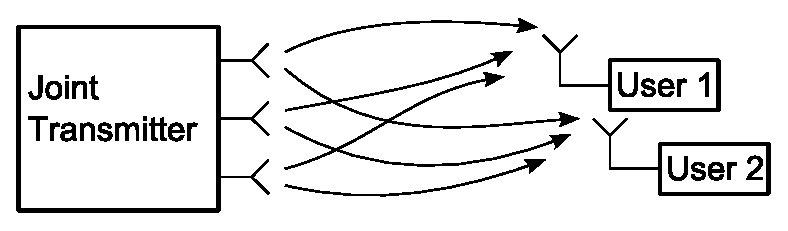
\includegraphics[scale=0.8]{BC}
		\end{figure}	
	\end{itemize}
	\item Advantage of multiuser MIMO compared to point\,-\,to\,-\,point MIMO
	\begin{itemize}
		\item multiplexing gain can be exploited even if users have only single antenna
		\item users are spatially distributed in cell $\rightarrow $ channels to different users are independent
	\end{itemize}
\end{itemize}
\subsection{Multiple Access Channel (MAC)}
We consider two aspects:
\begin{itemize}
	\item Detector structures
	\item Rate region
\end{itemize}
\subsubsection{Detector structures}
\paragraph*{Channel model:}
\textbf{Bild einf\"ugen und diese Zeile l\"oschen}\\
$\rightarrow  $ general MAC: $\mathbf{y} = \sum\limits_{k = 1}^{K}\mathbf{H}_k\mathbf{x}_k + \mathbf{n} $\\
with: \begin{itemize}
	\item K users
	\item user $k $ has $N_{T,k} $ transmit antennas
	\item $N_R $ receive antennas
	\item $\mathbf{H}_k \in \mathbb{C}^{N_R\times N_{T,k}} $ 
\end{itemize}
\begin{align*}
	\mathbf{y} = 
	\underbrace{
	\begin{bmatrix}\mathbf{H}_1 & \mathbf{H}_2 & \ldots & \mathbf{H}_k 	
	\end{bmatrix}
	}_{\mathbf{H}}\cdot
	\underbrace{
	\begin{bmatrix}\mathbf{x}_1 \\ \vdots \\ \mathbf{x}_k		
	\end{bmatrix}}_{\mathbf{x}} + \mathbf{n}
\end{align*}
\paragraph*{Observation:}
\begin{itemize}
	\item same equivalent channel model as for a point\,-\,to\,-\,point MIMO system transmitting $N_T = \sum_{k = 1}^{K} N_{T,k} $ independent signal streams \quad \textit{(Anmerkung: kein Unterschied f\"ur Empf\"anger, ob Signale von einem Nutzer oder von mehreren)}
	\item the receiver (e.g. base station) can use detection schemes as for point\,-\,to\,-\,point MIMO systems
	\begin{itemize}
		\item linear receiver
		\item DFG
		\item sphere decoder
	\end{itemize}
\end{itemize}
\paragraph*{Typical problems in uplink multiuser MIMO}
For given receiver structure:
\begin{itemize}
	\item calculate $\text{SNR}_k $ for all users $k $ based on the expressions developed in Chapter 2.4
	\item optimize transmit power of users, $E_k = \mathcal{E}\bigl\{||x_k||^2\bigr\} $ for maximization of the sumrate or maximization of the minimum $\text{SNR}_k $ \quad \textit{(Anmerkung: Maximierung der \textit{sumrate} kann durch Maximierung des SNR des Users mit bestem Kanal erfolgen, aber: unfair anderen Usern gegen\"uber $\Rightarrow $ \textit{starving})}
\end{itemize}
\subsubsection{Rate region}
For point\,-\,to\,-\,point links, we can decode error free, if the rate, $R$, meets
  \begin{itemize}
     \item[a)] SISO	$R < \log_2\bigl(1+\frac{\mathcal{E}_s}{\sigma_n^2}	\bigr) $
     \item[b)] MIMO $R < \log_2\underbrace{\bigl|\mathbf{I} + \frac{\mathcal{E}_s}{N_T\sigma_n^2} \mathbf{HH}^H\bigr|}_{\text{det}} $
	\end{itemize} 
Questions: What happens if there are multiple users?
\paragraph{Rate Region for Single Antenna Users and Receivers}
\begin{itemize}
	\item Gaussian channel
	\item $N_R = N_{T,k} = 1 \forall	k $
	\item received signal: 
	\begin{align*}
		y &= \sum\limits_{k = 1}^{K}x_k + n\\ * \mathcal{E}_k &= \mathcal{E}\bigl\{||x_k||^2\bigr\} \\ *\sigma_n^2 &= \bigl\{||n||^2\bigr\}
	\end{align*}
\end{itemize}
\subparagraph*{Example: 2 Users}
\textbf{Bild einf\"ugen und diese Zeile l\"oschen}
\begin{itemize}
	\item How should we choose $R_1 $ and $R_2 $ to ensure error free decoding of \underline{both} signal streams?
	\item It is no longer sufficient to maximizie a single rate. Instead we have to consider rate pairs $(R_1, R_2)$
	\item All possible rate points, that allows error free decoding, define the rate region $\underline{C} $
	\item Possible desing goals of the system:
	\begin{itemize}
		\item maximized sumrate $R_{\text{sum}} = \underset{(R_1, R_2) \in \underline{C}}{\text{max}} R_1 + R_2 $ 
		\item maximize minimum user rate: $R_{\text{max-min}} = \underset{(R_1, R_2) \in \underline{C}}{\text{max}} \, \underset{i \in \{1, 2\}}{\text{min}} R_i $ 
	\end{itemize}
	\item Rate Region of two user Gaussian MAC \quad\textit{Anmerkung: Einschr\"ankungen}
	\begin{align}
		R_1 &< \log_2\bigl(1 + \frac{\mathcal{E}_1}{\sigma_n^2}\bigr) \label{eq:Formel_1}\\ 
		R_2 &< \log_2\bigl(1 + \frac{\mathcal{E}_2}{\sigma_n^2}\bigr)\label{eq:Formel_2} \\ 
		R_1 + R_2 &< \log_2\bigl(1 + \frac{\mathcal{E}_1 + \mathcal{E}_2}{\sigma_n^2}\bigr) 	\label{eq:Formel_3}	
	\end{align}
	\item Interpretation:
	\begin{itemize}
		\item \eqref{eq:Formel_1} and \eqref{eq:Formel_2}  (= single\,-to\,user constraint) are the ``single\,-\,user bounds´´, i.e., the maximum rates of user 1 and 2, if the other user was not there
		\item \eqref{eq:Formel_3} can be interpreted as the maximum rate if streams of users 1 and 2 were jointly encoded. The separate encoding in the MAC cannot yield a better performance
		\item Graphical represantation: \textbf{Bild einf\"ugen und diese Zeile l\"oschen}
	\end{itemize}
\end{itemize}
\end{document}
